\section{Spectre}
In 2018, Gruss et al.\cite{spectre} proposed the new Spectre attack on Intel/AMD processors. The root cause of Spectre and its variants lies on the implicit state transformation in cache. When an instruction is executed speculatively due to the branch prediction, it's expected that all states before the speculation will be resumed. However, the discard of store-load instruction will not roll back the states in cache, indicating that the data speculatively brought to cache will stay in cache. This causes information leakage if the data is sensitive.

The attack is verified on x86 and ARM machines. However, the attack depends on several primitive components in architecture such as the timer, cache and branch predictor. And yet there's no valid proof-of-concept attack on XiangShan. Our goal is to develop the Spectre attack primitive on XiangShan core.

\subsection{Spectre on x86 and ARM}
The Spectre attack assumes that the attacker and victim shares the same cache but in different core. The victim has a similar code snippet like

\begin{listing}[!h]
\begin{minted}{c}
uint8_t array[160] = {1, 2, ..., 16};
char* secret = "Secret goes here!";

void victim_function(size_t x) {
   if (x < array1_size) { // array1_size = 16
       temp &= array2[array1[x] * CACHELINE_SIZE];
   }
}
\end{minted}
\label{listing:spectre_vulnerable}
\caption{Vulnerable code in victim}
\end{listing}

The attacker has access to \verb|array2| and then train the branch predictor with legal input \verb|x|. After sufficient training,
the branch predictor will always predict the branch in victim function to be taken. So next time a caller invokes the victim function,
the speculative engine will try to execute instructions inside if statement, even if it's out of bound.

\begin{listing}[!h]
\begin{minted}{c}
for (int x = 0; x < ENTRY_SIZE; ++x) {
    victim_function(x);
}
flush_cache(array2);
victim_function(secret[i++]);

for (int i = 0; i < 256; i++) {
    addr = &array2[i * CACHELINE_SIZE];
    time1 = __rdtscp(&junk); /* READ TIMER */
    junk = * addr; /* MEMORY ACCESS TO TIME */
    time2 = __rdtscp(&junk) - time1; 
    /* READ TIMER & COMPUTE ELAPSED TIME */
    if (time2 <= CACHE_HIT_THRESHOLD)
        results[i]++;
}

\end{minted}
\label{listing:training-bp}
\caption{Training the branch predictor}
\end{listing}

To carry out the leak information, an attacker often adapts a probe array, i.e., \verb|array2| in this example. The array is used to detect which element is loaded into cache, because the secret information is encoded to be the offset. A detail goes here: the offset accessed in \verb|array2| must be a multiple of \verb|CACHELINE_SIZE| because if the offset is less, we are blinded to it. Adjacent data might be mapped to the same cache line and therefore, we are not able to tell that difference.

In real-world scenario, address of secrets can be in the kernel and attacker has to look for vulnerable snippets shown in \href{listing:spectre_vulnerable}{Listing 1}.

\subsection{Spectre on XiangShan}

The Spectre seems to work on XiangShan, and only a few tweaks need to be made to migrate. However, the branch predictor technology has advanced
for a great leap in these years.

\subsubsection{Branch Predictor}
Nanhu, the $2^{\text{th}}$ architecture of XiangShan, has $\mu$BTB, BTB, TAGE, RAS and Loop Predictor integrated in its branch predictor.

\begin{figure}[!htbp]
    \centering
    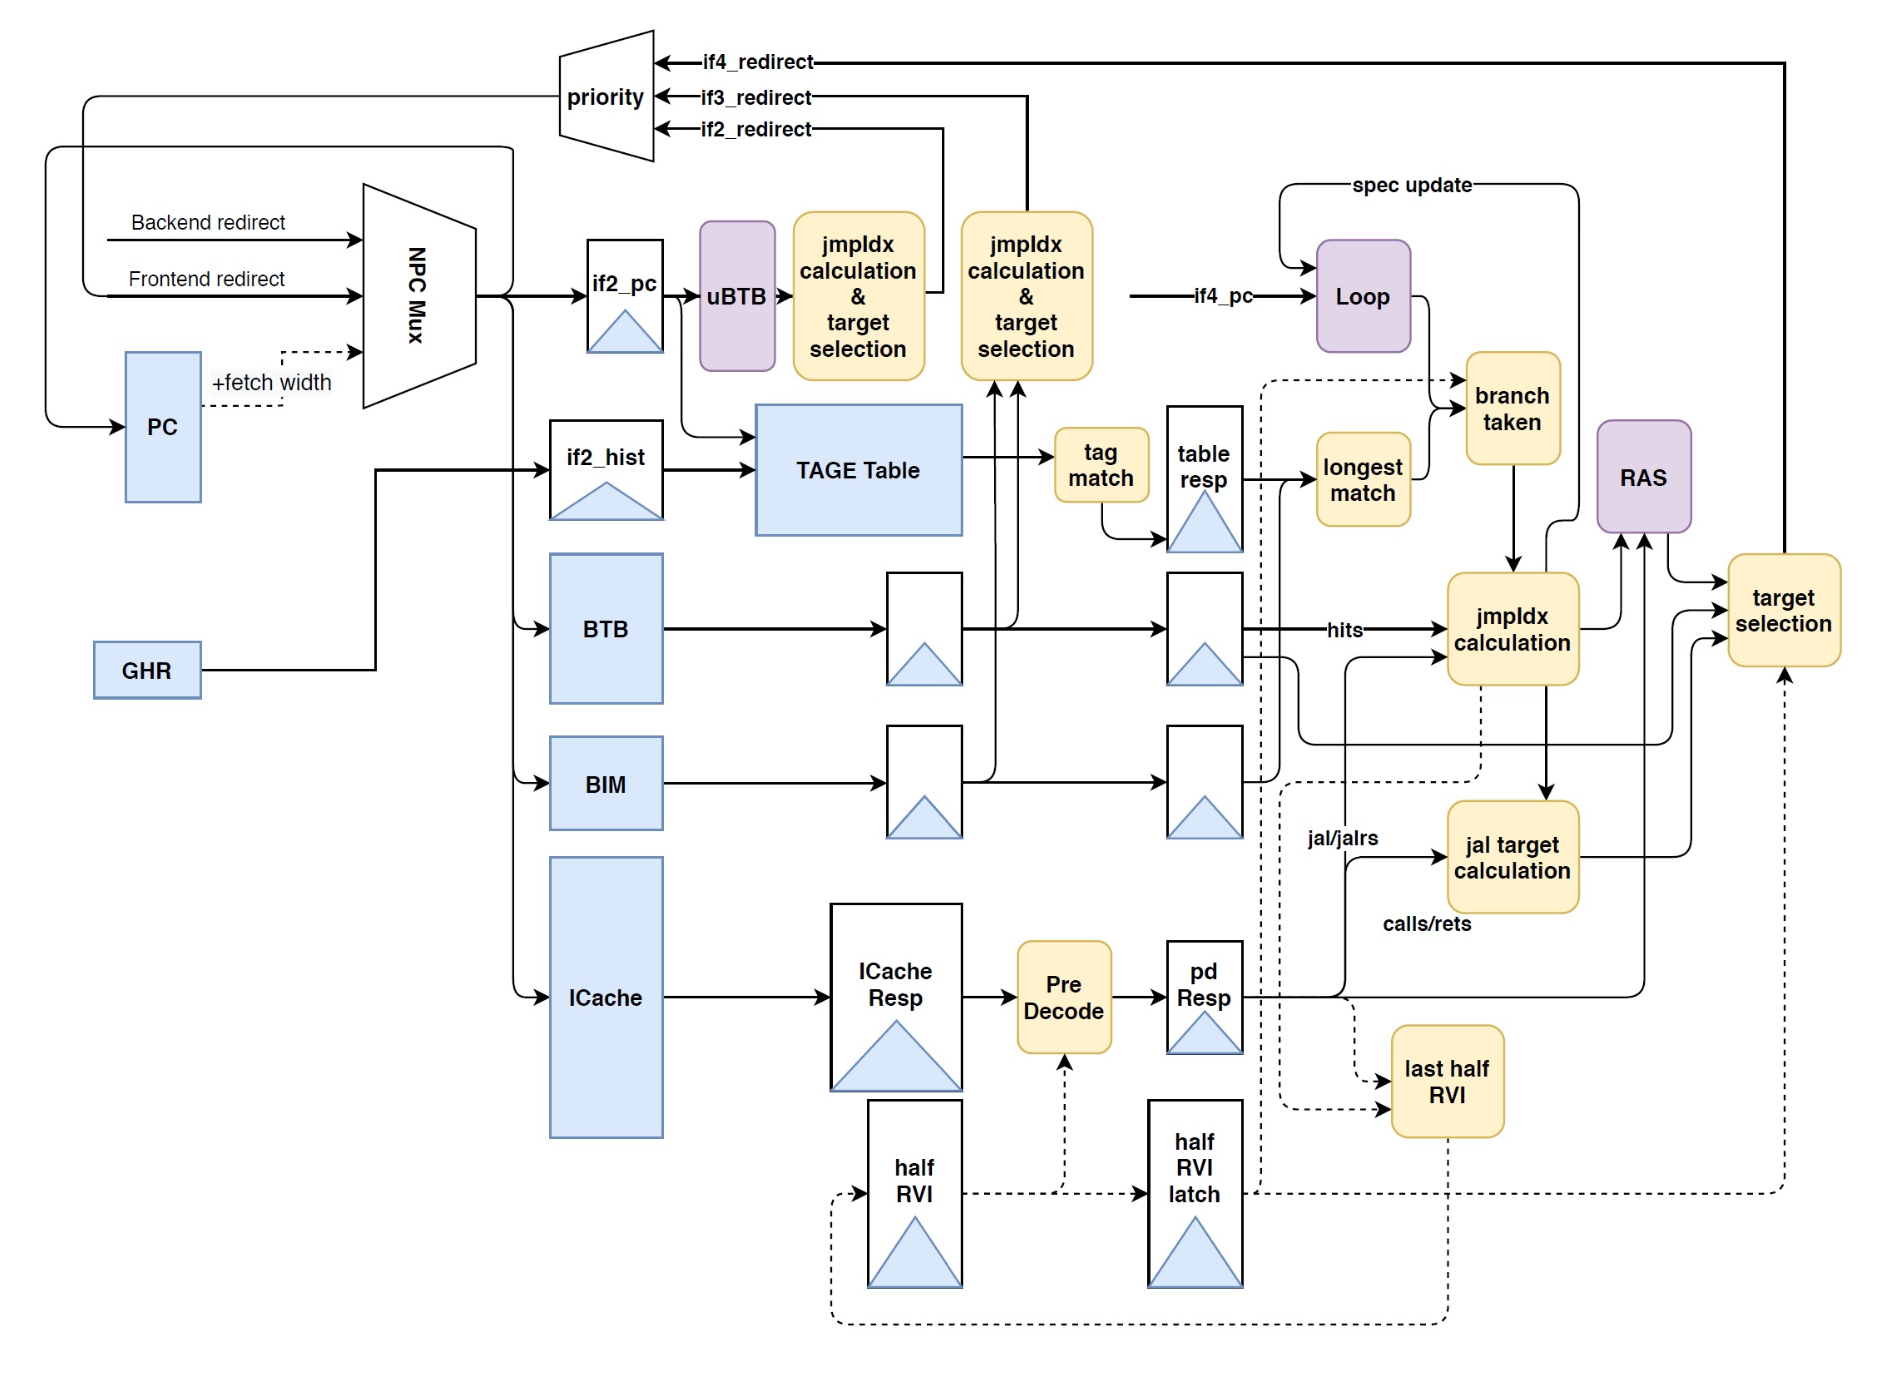
\includegraphics[width=0.99\linewidth]{Figure/xs-branch-predictor.png}
    \caption{Branch predictor design of Nanhu}
    \label{fig:xs-branch-pred}
\end{figure}

Among the components, TAGE with Loop Predictor is the top concerned for disabling the traditional Spectre attacks. TAGE is a global predictor with
context information hashed into a tag. Most time it cooperates with loop predictor to enhance the accuracy, since most of the branches are actually the exit conditon of a loop. If the predictor can recognize that loop, it can skip the meaningless prediction.

However, this feature mitigates Spectre in \href{listing:training-bp}{Listing 2}, by recognizing the loop and calling context in the training procedure and predicts that, in the next line when attack accesses the out-of-bound, the branch result is false.

\subsubsection{Cache}
Table 1 shows the default parameters of Nanhu architecture. Obviously, we need to tune the parameter in the above listing to the numbers shown below.

\begin{table}[!htbp]
	\centering
	\begin{tabular}[c]{ll}
		\toprule
        Parameter & Value \\
		\midrule
        L1 Sets & 256 \\
        L1 Ways & 8 \\
        L1 Linesize & 64 bytes \\
        Cache alias & Virtual Index Physical Tag \\
		\bottomrule
	\end{tabular}
    \caption{L1 Cache parameters}
\end{table}

In cache eviction, we needs to create 8 trash variable with the same index (the bits from 7th to 14th), and the \verb|CACHELINE_SIZE| is set to be 64. Meanwhile, the L1 sets number ensures that all ASCII character can be encoded and VIPT (Virtual Index Physical Tag) cache alias indicates that virtual address is enough for our exploitation.

\subsubsection{Attack on Nanhu}
Based on the discovery, we tweaks our exploitation to the listing shown below

\begin{listing}[!h]
\begin{minted}{c}
for (int i = 0; i <= ENTRY_SIZE; ++i) {
    int x = i < ENTRY_SIZE ? i : secret[i++]
    flush_cache(array2);
    victim_function(x);
}

for (int i = 0; i < 256; i++) {
    addr = &array2[i * CACHELINE_SIZE];
    time1 = rdcycle(); /* READ TIMER */
    junk = * addr; /* MEMORY ACCESS TO TIME */
    time2 = rdcycle() - time1; 
    /* READ TIMER & COMPUTE ELAPSED TIME */
    if (time2 <= CACHE_HIT_THRESHOLD)
        results[i]++;
}
\end{minted}
\label{listing:spectre-nanhu}
\caption{Spectre on Nanhu}
\end{listing}

The major change is that we combine the final access to secret to the training.
Actually, it is not the real implementation, since the second line involves a branch, but it could be optimized into a table array, which is trivial.
Another change is the access to timer, in RISC-V ISA, the instruction to read a timer is \verb|rdcycle|.

\subsection{Mitigation}

So far, most of the mitigation techniques are validated on RISC-V. Khasawneh et al.\cite{safespec} proposed a temporary buffer called SafeSpec, to store
the data before the instruction commits. To avoid another timing difference in that buffer, 
SafeSpec won't forward its internal data, so as to disable cache-based side channel attacks. However, this introduces 5 percent performance overhead and more circuits in chips.

An improvement was present by SpectreGuard \cite{spectreguard} and SpecTerminator \cite{specterminator}. These works proposed techniques to 
detect possible vulnerable code snippet and transient window, and then mark with tags to prevent them from being loaded into cache before committing instruction.